%% FERMI SEA SPHERE
% https://latexdraw.com/draw-a-sphere-in-latex-using-tikz/

\documentclass{standalone}



\IfStandalone{\def\datapath{../../../}}{\def\datapath{}}


\IfStandalone{\def\datapath{../../../}}{\def\datapath{}}

\usepackage{xcolor}
\definecolor{SciencePurple}{HTML}{663399}
\definecolor{ScienceBlue}{HTML}{214CCE}
\definecolor{ScienceGreen}{HTML}{007510}
\definecolor{ScienceYellow}{HTML}{ffbf00}
\definecolor{ScienceOrange}{HTML}{ff8c00}
\definecolor{ScienceRed}{HTML}{dc143c}
\usepackage{fontspec}
	\setmainfont{Roboto Slab}
	\setsansfont{Lato}
	\renewcommand{\familydefault}{\sfdefault}
	\setlength{\intextsep}{4pt} % Set defualt spacing around floats
	\definecolor{CommentGreen}{HTML}{228B22}
%	\captionsetup{aboveskip=5pt, belowskip=5pt} % Reduce space around captions

%% Math Env Text Settings
\usepackage{mathtools}
\usepackage{unicode-math}
	\setmathfont{XITS Math}
\usepackage{amsmath}
\usepackage{bm}
%	\everymath=\expandafter{\the\everymath\displaystyle}


%% https://tex.stackexchange.com/questions/8434/how-to-scale-math-font-only#8448
\DeclareMathSizes{11pt}{12pt}{7pt}{7pt}
\DeclareMathSizes{14pt}{15pt}{9pt}{9pt}

%% https://tex.stackexchange.com/questions/122574/globally-changing-math-line-spacing
\setlength{\jot}{7pt}

%% https://www.overleaf.com/learn/latex/Spacing_in_math_mode
%% https://tex.stackexchange.com/questions/41913/how-to-get-less-spacing-in-math-mode
%% https://mirror.kumi.systems/ctan/obsolete/info/math/voss/mathmode/Mathmode.pdf
\thinmuskip=5mu % (by default it is equal to 3 mu)
\medmuskip=5mu  % (by default it is equal to 4 mu)
\thickmuskip=7mu  % (by default it is equal to 5 mu)


\usepackage{tikz}
\usepackage{siunitx}
\usepackage{pgfplots}

\usepackage{physics}
\usepackage{etoolbox} %ifthen
\usepackage[outline]{contour} % glow around text


%%%%%%%%%% PGFPLOTS & PGFPLOTS SETTINGS %%%%%%%%%%
\pgfplotsset{compat=newest,
	width=6cm,
	height=3cm,
	scale only axis=true,
	max space between ticks=25pt,
	try min ticks=5,
	every axis/.style={
		axis y line=left,
		axis x line=bottom,
		axis line style={thick,->,>=latex, shorten >=-.4cm}
	},
	every axis plot/.append style={thick},
	tick style={black, thick}
}
\tikzset{
	semithick/.style={line width=0.8pt},
}

\usepgfplotslibrary{groupplots}
\usepgfplotslibrary{dateplot}

% https://tex.stackexchange.com/questions/441917/is-there-a-simple-way-to-use-stick-figures-into-pgf-tikz-drawings
\usepackage{tikzsymbols}
\usetikzlibrary{shapes.symbols}

\usetikzlibrary{calc}
\usetikzlibrary{arrows,arrows.meta,math}
\usetikzlibrary{decorations.markings}
\usetikzlibrary{angles,quotes} % for pic (angle labels)
\usetikzlibrary{fadings}

% https://tikz.dev/library-3d
\usetikzlibrary{3d}

% https://latexdraw.com/draw-a-sphere-in-latex-using-tikz/
\usepackage{tikz-3dplot}

% Define Color
\tikzstyle{bigphoton}=[-{Latex[length=8,width=6]},red!95!black!50,opacity=0.85,very thin,decorate,decoration={snake,amplitude=2.8,segment length=8,post length=8}]

\contourlength{1.4pt}




\begin{document}
	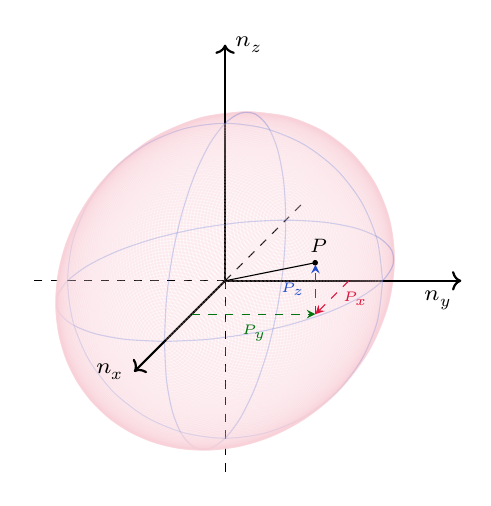
\begin{tikzpicture}
		% Parametric equations of the sphere
		\tikzmath{function equis(\r,\p,\t) {return \r * sin(\p r) * cos(\t r);};}
		\tikzmath{function ye(\r,\p,\t) {return \r * sin(\p r) * sin(\t r);};}
		\tikzmath{function zeta(\r,\p,\t) {return \r * cos(\p r);};}
		\pgfmathsetmacro{\tcero}{0.0}
		\pgfmathsetmacro{\phiInit}{0.0}
		\pgfmathsetmacro{\phiMid}{0.5*pi}
		\pgfmathsetmacro{\phiEnd}{pi}
		\pgfmathsetmacro{\thetaInit}{0.5*pi}
		\pgfmathsetmacro{\thetaMid}{1.85*pi}
		\pgfmathsetmacro{\thetaEnd}{2.5*pi}
		
		%
		
		\pgfmathsetmacro{\step}{0.02}
		\pgfmathsetmacro{\next}{\tcero+0.5*\step}
		\pgfmathsetmacro{\sig}{2.0*\step}
		\pgfmathsetmacro{\radio}{2.0}
		\pgfmathsetmacro{\sigP}{\phiMid+\step}
		\pgfmathsetmacro{\sigPp}{\sigP+\step}
		
		
		% Part of the z axis below the sphere
		\draw[dashed] (0,0,-1.25*\radio) -- (0,0,-\radio);
		
		% I start to draw the sphere from below
		% Part of the sphere under the plane z = 0
		\foreach \p in {\sigP,\sigPp,...,\phiEnd}{
			\draw[ScienceRed!20,thick,opacity=0.25] plot[domain=\thetaInit:\thetaEnd,smooth,variable=\t] 
			({equis(\radio,\p,\t)},{ye(\radio,\p,\t)},{zeta(\radio,\p,\t)}); 
		}
		
		% Then I draw the part of the coordinate axis that is inside the sphere. 
		%%% Coordinate axis
		\draw[thick,->] (0,0,0) -- (1.5*\radio,0,0) node [below left] {\footnotesize$n_y$};
		\draw[dashed] (0,0,0) -- (-1.25*\radio,0,0);
		\draw[thick,->] (0,0,0) -- (0,1.5*\radio,0) node [right] {\footnotesize$n_z$};
		\draw[dashed] (0,0,0) -- (0,-1.25*\radio,0);
		\draw[dashed] (0,0,0) -- (0,0,-\radio);
		
		% As a reference, I draw a circumference at z = 0 (phi = pi / 2).
		\draw[ScienceBlue,opacity=0.25] plot[domain=0:2*pi,smooth,variable=\t] 
		({equis(\radio,\phiMid,\t)},{ye(\radio,\phiMid,\t)},{zeta(\radio,\phiMid,\t)});
		
		% As a reference, I draw a circumference at x = 0 (theta = 0).
		\draw[ScienceBlue,opacity=0.25] plot[domain=0:2*pi,smooth,variable=\t] 
		({equis(\radio,\t,0)},{ye(\radio,\t,0)},{zeta(\radio,\t,0)});
		
		% As a reference, I draw a circumference at y = 0 (theta = pi/2).
		\draw[ScienceBlue,opacity=0.25] plot[domain=0:2*pi,smooth,variable=\t] 
		({equis(\radio,\t,\thetaInit)},{ye(\radio,\t,\thetaInit)},{zeta(\radio,\t,\thetaInit)});
		
		
		%
		% Now I draw the part of the sphere that is behind the axis
		%
		\foreach \p in {\step,\sig,...,\phiMid}{
			\draw[ScienceRed!20,thick,opacity=0.25] plot[domain=\thetaInit:\thetaMid,smooth,variable=\t] 
			({equis(\radio,\p,\t)},{ye(\radio,\p,\t)},{zeta(\radio,\p,\t)}); 
		}
		
		
		% Z axis that is inside the sphere
		% This part has to be in front of the rear part of the sphere
		\draw[thick] (0,0,0) -- (0,0,\radio);
		
		
		%
		% Sphere (the part that is in front of the z axis)
		%
		\foreach \p in {\step,\sig,...,\phiMid}{
			\draw[ScienceRed!20,thick,opacity=0.25] plot[domain=\thetaMid:\thetaEnd,smooth,variable=\t] 
			({equis(\radio,\p,\t)},{ye(\radio,\p,\t)},{zeta(\radio,\p,\t)}); 
		}
		
		
		% Part of the z axis that is above the sphere
		\draw[thick,->] (0,0,\radio) -- (0,0,1.5*\radio) node [left] {\footnotesize $n_x$};
		
		
		% Create a point (P)
		\coordinate (P) at ({0.5*pi},{0.2*pi},{0.35*pi});
		\coordinate (P2) at ({0.51*pi},{0.21*pi},{0.35*pi});
		% Line from the origin to (P)
		\draw[-{Circle[length=2pt]}] (0,0,0) -- (P2) node[above] {\scriptsize $P$};
		
		
		
		
		% Create a point (Pxy)
		\coordinate (Pxy) at ({0.5*pi},0,{0.35*pi});
		
		% Create a point (Px)
		\coordinate (Px) at ({0.5*pi},0,0);
		% Line from axis start (Px) to Pxy
		\draw[-{stealth[length=0.5pt]},dashed,ScienceRed] (Px) -- (Pxy) node[midway,below=0.5,right=0.5] {\tiny $P_x$};
		
		% Create a point (Py)
		\coordinate (Py) at (0,0,{0.35*pi});
		% Line from axis start (Px) to Pxy
		\draw[-{stealth[length=0.5pt]},dashed,ScienceGreen] (Py) -- (Pxy) node[midway,below=0.5] {\tiny $P_y$};
		
		% Dotted line to project from Pxy to P
		\draw[-{stealth[length=0.5pt]},dashed,ScienceBlue] (Pxy) -- (P) node[midway,left=0.5] {\tiny $P_z$};
		
		
	%	% Create a point (P)
	%	\coordinate (Py) at ({0.5*pi},{0},{0});
	%	% Line from the origin to (P)
	%	\draw[-stealth,dashed] ({0.5*pi},{0.5*pi},0) -- (Py) node[midway] {\tiny $P_y$};
	%	
	\end{tikzpicture}
\end{document}